% Autor: Simon May
% Datum: 2014-08-19

% 1. Teil der Überschrift rechtsbündig
% (eckige Klammern: Eintrag im Inhaltsverzeichnis)
\section[Lageplan des naturwissenschaftlichen Zentrums (NWZ)]{\raggedleft Lageplan des naturwissen-}
% Lageplan (links) als Hintergrund auf der 1. Seite
\begin{tikzpicture}[remember picture, overlay]
\node[inner sep=0, xshift=0.9cm, yshift=-0.5cm] at (current page.center)
{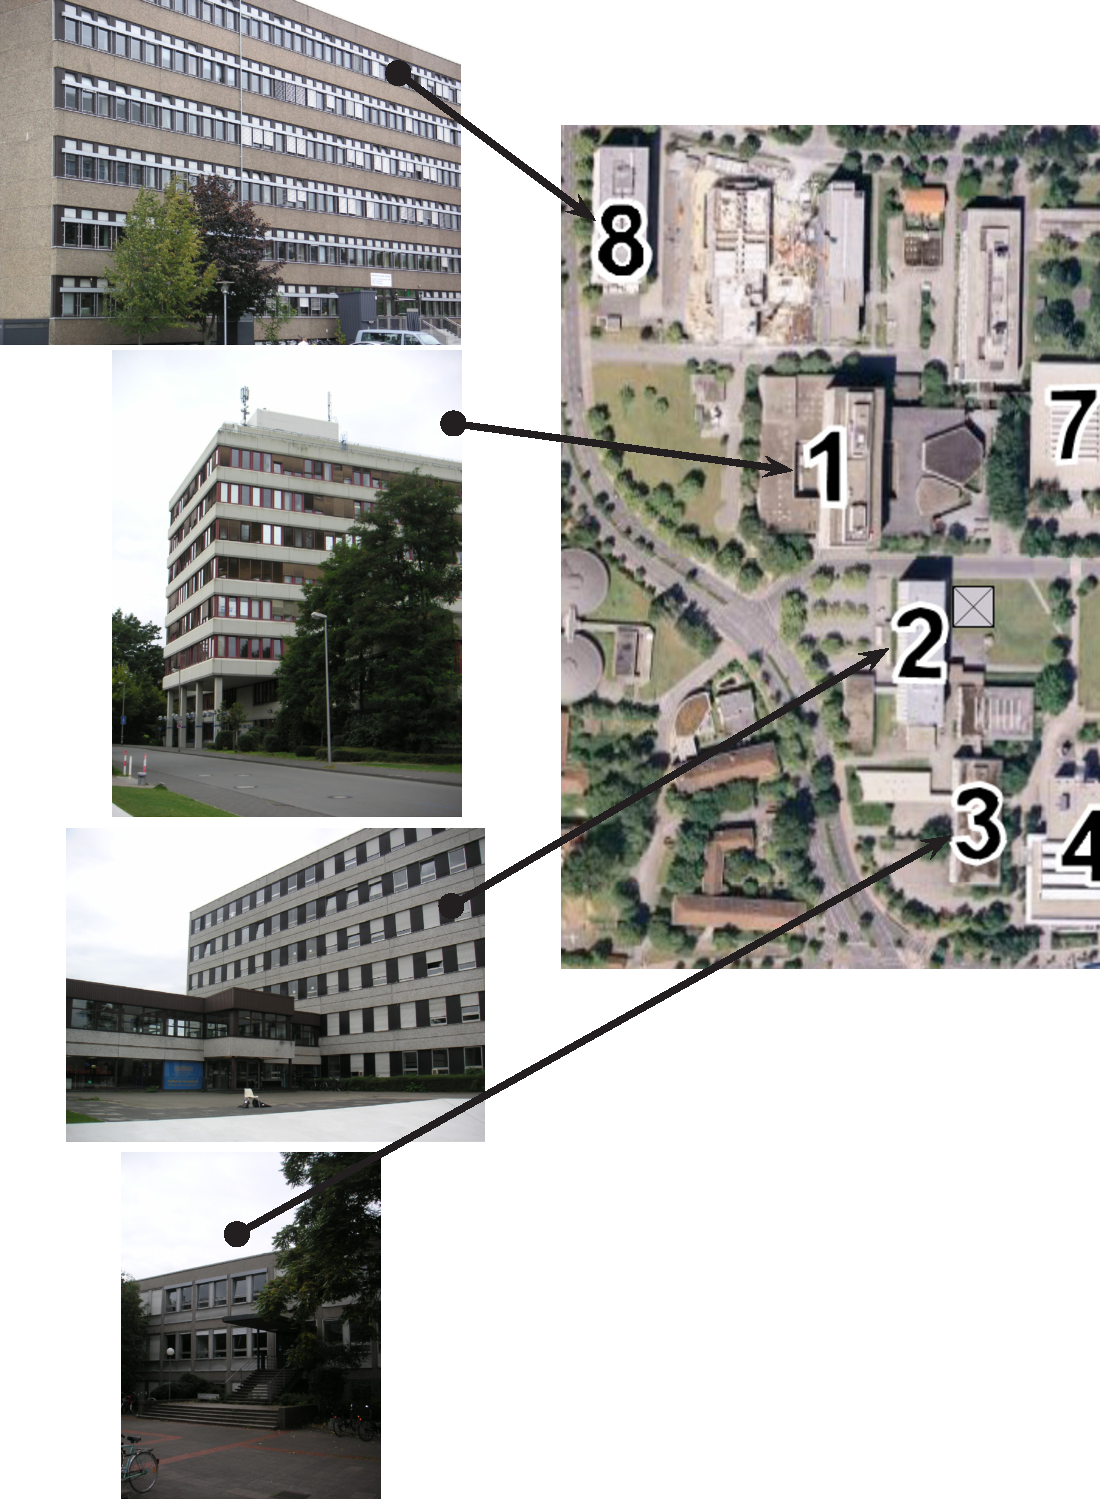
\includegraphics{res/lageplan_links.pdf}};
\end{tikzpicture}

\vspace{\fill}
{\large
\begin{enumerate}
\hfill\begin{minipage}{8.7cm}
\item Institutsgruppe~1~(IG~1) mit:
	\begin{itemize}[leftmargin=0.4cm]
	\item Physikalisches Institut (PI)
	\item Institut für Festkörpertheorie (FT)
	\item Institut für Materialphysik (MP)
	\item Institut für Didaktik der Physik~(DP)
	\item Technik und Sachunterricht (TS)
	\end{itemize}
\item Kernphysik-Gebäude
	\begin{itemize}[leftmargin=0.4cm]
	\item Institut für Kernphysik (KP)
	\item Institut für theoretische Physik (TP)
	\end{itemize}
\item Angewandte Physik (AP)
\end{minipage}
\end{enumerate}

\clearpage
% 2. Teil der Überschrift linksbündig
\section*{\raggedright schaftlichen Zentrums (NWZ)}
% Lageplan (rechts) als Hintergrund auf der 2. Seite
\begin{tikzpicture}[remember picture, overlay]
\node[inner sep=0, xshift=-0.6cm, yshift=0.22cm] at (current page.center)
{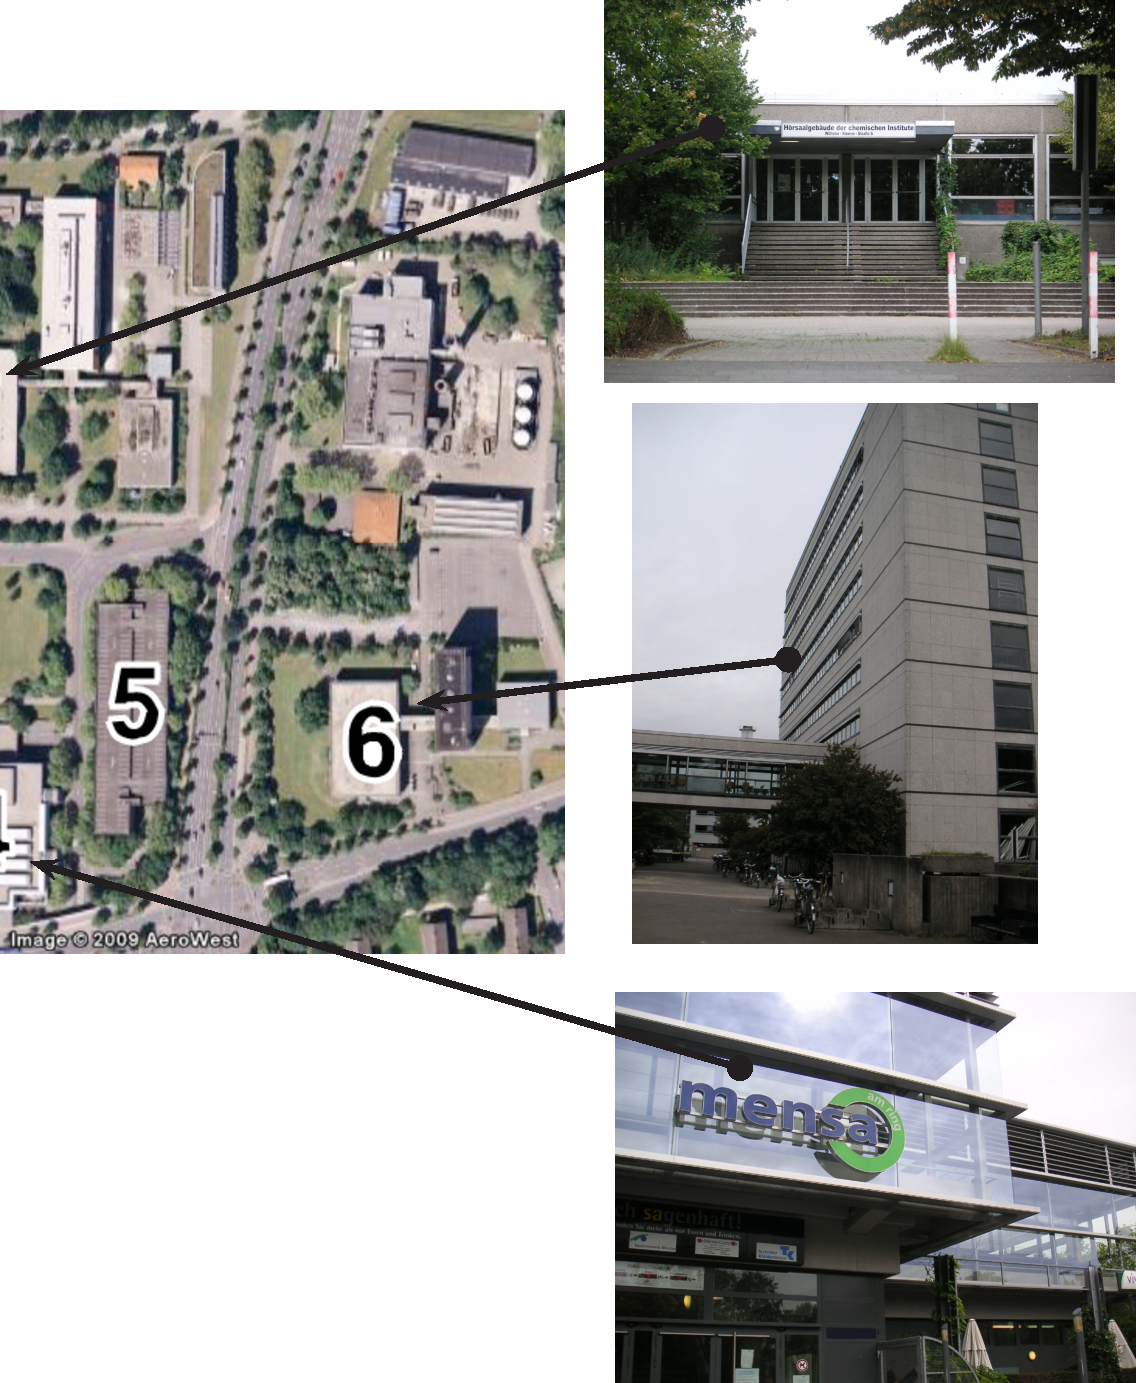
\includegraphics{res/lageplan_rechts.pdf}};
\end{tikzpicture}


\vspace{\fill}
% "resume": Nummerierung fortsetzen
\begin{enumerate}[resume]
\begin{minipage}{8.2cm}
\item Mensa + Viva-Café
\item Parkhaus
\item Mathematische Institute
	\begin{itemize}[leftmargin=0.4cm]
	\item Institut für angewandte Mathematik
	\item Institut für reine Mathematik
	\item Institut für Logik
	\item Zentrum für Informationsverarbeitung (ZIV)
	\end{itemize}
\item Chemie
\item Institut für Geophysik
\end{minipage}
\end{enumerate}
}
